\documentclass[12pt,aspectratio=169]{beamer}
\usepackage{amsmath, amssymb}
\usepackage{booktabs}
\usepackage{tikz}
\usetikzlibrary{arrows.meta,decorations.pathmorphing,patterns,calc,shadings}
\usepackage{pgfplots}
\pgfplotsset{compat=1.18}
\usepackage{xcolor}
\usepackage{array}


% ── Theme (identical to WSR / PFR decks) ───────────────────────────────
\usetheme{Madrid}
\definecolor{firered}{RGB}{180,30,10}
\definecolor{ashgrey}{RGB}{50,55,65}
\definecolor{skyblue}{RGB}{30,100,180}
\definecolor{flameyellow}{RGB}{230,155,15}
\setbeamercolor{palette primary}{bg=ashgrey,fg=white}
\setbeamercolor{palette secondary}{bg=ashgrey!85,fg=white}
\setbeamercolor{palette tertiary}{bg=ashgrey!65,fg=white}
\setbeamercolor{palette quaternary}{bg=ashgrey,fg=white}
\setbeamercolor{structure}{fg=skyblue}
\setbeamercolor{alerted text}{fg=firered}
\setbeamercolor{block title}{bg=skyblue,fg=white}
\setbeamercolor{block body}{bg=skyblue!8}
\setbeamercolor{block title alerted}{bg=firered,fg=white}
\setbeamercolor{block body alerted}{bg=firered!10}
\setbeamercolor{block title example}{bg=ashgrey,fg=white}
\setbeamercolor{block body example}{bg=ashgrey!10}
\setbeamerfont{title}{size=\Large,series=\bfseries}
\setbeamertemplate{navigation symbols}{}
\setlength{\itemsep}{1pt}

% ── Macros ──────────────────────────────────────────────────────────────
\newcommand{\Da}{\mathrm{Da}}
\newcommand{\Le}{\mathrm{Le}}
\newcommand{\Pe}{\mathrm{Pe}}
\newcommand{\ddx}[1]{\frac{d#1}{dx}}
\newcommand{\ddt}[1]{\frac{d#1}{dt}}
\newcommand{\pd}[2]{\frac{\partial #1}{\partial #2}}
\newcommand{\Tad}{T_{\text{ad}}}
\newcommand{\Tu}{T_u}
\newcommand{\Tb}{T_b}
\newcommand{\Tf}{T_f}
\newcommand{\mdot}{\dot{m}}
\newcommand{\wdot}{\dot{\omega}}
\newcommand{\SL}{S_L}
\newcommand{\lf}{\delta_f}
\newcommand{\tchem}{t_{\text{chem}}}
\newcommand{\tdiff}{t_{\text{diff}}}
\newcommand{\Ma}{\mathrm{Ma}}
\newcommand{\Yf}{Y_F}
\newcommand{\alphath}{\alpha}

% ════════════════════════════════════════════════════════════════════════
\title{Laminar Premixed Flames}
\subtitle{Structure, Flame Speed, and Aeronautical Applications}
\author{Prof.Dr. Onur Tuncer}
\institute{Istanbul Technical University}
\date{\today}

\begin{document}

\begin{frame}
  \titlepage
\end{frame}

\begin{frame}{Lecture Outline}
  \tableofcontents
\end{frame}

% ════════════════════════════════════════════════════════════════════════
\section{What is a Premixed Flame?}
% ════════════════════════════════════════════════════════════════════════

\begin{frame}{Premixed vs.\ Diffusion Flames: A Fundamental Distinction}

  \begin{columns}
    \begin{column}{0.50\textwidth}
      \begin{block}{Premixed flame}
        \begin{itemize}
          \item Fuel and oxidiser \textbf{mixed before} the reaction zone
          \item Single, well-defined flame front propagates into
                the unburned mixture
          \item Propagation speed controlled by
                \emph{chemistry and diffusion}
          \item Examples: spark-ignition engines, lean-premixed
                gas turbine burners, Bunsen burner (inner cone)
        \end{itemize}
      \end{block}
    \end{column}
    \begin{column}{0.46\textwidth}
      \begin{alertblock}{Diffusion (non-premixed) flame}
        \begin{itemize}
          \item Fuel and oxidiser meet \textbf{at} the reaction zone
          \item No distinct propagation speed; flame sits at
                stoichiometric surface
          \item Burn rate controlled by \emph{mixing}
          \item Examples: candle, jet engine main combustor
                (traditional), rocket engines
        \end{itemize}
      \end{alertblock}
    \end{column}
  \end{columns}

  \smallskip
  \begin{exampleblock}{Why premixed flames matter in aeronautics?}
    \small LPP gas turbine combustors, lean direct injection (LDI), and
    detonation-based engines all rely on premixed flame physics.
    Flash-back and auto-ignition are the critical safety limits.
  \end{exampleblock}
\end{frame}

\begin{frame}{The Laminar Premixed Flame: Physical Picture}

  \begin{center}
  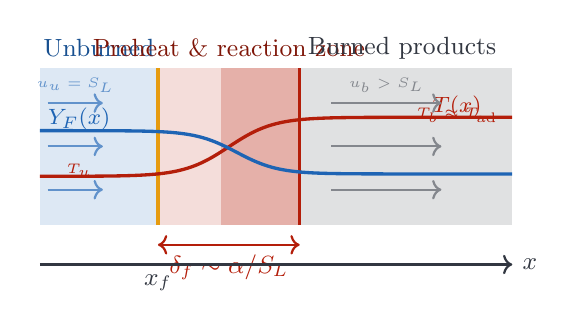
\begin{tikzpicture}[font=\small, scale=1.0]

    % Background zones
    \fill[skyblue!15] (-1.5,-1.0) rectangle (0.0, 1.0);
    \fill[firered!15] (0.0,-1.0)  rectangle (0.8, 1.0);
    \fill[firered!35] (0.8,-1.0)  rectangle (1.8, 1.0);
    \fill[ashgrey!15] (1.8,-1.0)  rectangle (4.5, 1.0);

    % Zone labels (top)
    \node[font=\small, skyblue!80!black] at (-0.75, 1.25)
      {Unburned};
    \node[font=\small, firered!70!black] at (0.9, 1.25)
      {Preheat \& reaction zone};
    \node[font=\small, ashgrey] at (3.1, 1.25)
      {Burned products};

    % Braces for flame thickness
    \draw[<->, thick, firered] (0.0,-1.25) -- (1.8,-1.25)
      node[midway, below, font=\small]{$\lf \sim \alpha/\SL$};

    % x-axis
    \draw[->, thick, ashgrey] (-1.5,-1.5) -- (4.5,-1.5)
      node[right]{$x$};
    \node[below, font=\small, ashgrey] at (0.0,-1.5) {$x_f$};

    % Flame-front marker
    \draw[very thick, flameyellow] (0.0,-1.0) -- (0.0,1.0);
    \draw[very thick, firered] (1.8,-1.0) -- (1.8,1.0);

    % T profile (sigmoidal, rising from left to right)
    \draw[firered, very thick, domain=-1.5:4.5, samples=200]
      plot(\x, {0.75*(1/(1+exp(-3.5*(\x-0.9)))) - 0.38});
    \node[firered, font=\footnotesize] at (3.8, 0.5) {$T(x)$};
    \node[firered, font=\tiny] at (-1.0,-0.3) {$\Tu$};
    \node[firered, font=\tiny] at (3.8, 0.4) {$\Tb \approx \Tad$};

    % Y_F profile (falling from left to right)
    \draw[skyblue, very thick, domain=-1.5:4.5, samples=200]
      plot(\x, {0.55*(1 - 1/(1+exp(-3.8*(\x-1.0)))) - 0.35});
    \node[skyblue, font=\footnotesize] at (-1.0, 0.35) {$\Yf(x)$};

    % Flow arrows (unburned side)
    \foreach \y in {-0.55, 0.0, 0.55}{
      \draw[->, skyblue!70, thick] (-1.4,\y) -- (-0.7,\y);
    }
    \node[skyblue!70, font=\tiny] at (-1.05, 0.78)
      {$u_u = \SL$};

    % Flow arrows (burned side, faster)
    \foreach \y in {-0.55, 0.0, 0.55}{
      \draw[->, ashgrey!60, thick] (2.2,\y) -- (3.6,\y);
    }
    \node[ashgrey!60, font=\tiny] at (2.9, 0.78)
      {$u_b > \SL$};

  \end{tikzpicture}
  \end{center}

  \vspace{-0.1cm}
  \small
  The flame front propagates at the \alert{laminar burning velocity} $\SL$
  into the unburned gas.
  Unburned gas ($\Tu$, $Y_{F,0}$) enters from the left;
  burned products ($\Tb \approx \Tad$) exit on the right at higher velocity
  (thermal expansion).
\end{frame}

% ════════════════════════════════════════════════════════════════════════
\section{Governing Equations}
% ════════════════════════════════════════════════════════════════════════

\begin{frame}{Governing Equations: 1-D Steady Premixed Flame}

  In the flame-fixed reference frame, the steady 1-D governing equations
  (constant pressure, Fickian diffusion) are:

  \medskip
  \textbf{Continuity:} $\quad \rho u = \rho_u \SL = \mdot'' = \text{const}$

  \medskip
  \textbf{Species:}
  \[
    \mdot'' \ddx{Y_k}
    = \ddx{}\!\left(\rho D_k \ddx{Y_k}\right) + \wdot_k W_k
  \]

  \textbf{Energy:}
  \[
    \mdot'' c_p \ddx{T}
    = \ddx{}\!\left(\lambda \ddx{T}\right)
      - \sum_k h_k \wdot_k W_k
  \]

  \begin{block}{Comparison with PFR (Unit 5)}
    The PFR \emph{dropped} the diffusion terms $d(\lambda\,dT/dx)/dx$
    and $d(\rho D_k\,dY_k/dx)/dx$ (high-Pe assumption).
    The premixed flame \textbf{retains} them --- diffusion is what
    allows the flame to propagate \emph{against} the flow.
    Without diffusion, $\SL = 0$.
  \end{block}
\end{frame}

\begin{frame}{Non-Dimensionalisation: The Zeldovich--Frank-Kamenetskii (ZFK) Framework}

  Introduce non-dimensional temperature $\theta = (T - \Tu)/(\Tad - \Tu)$
  and progress variable $c = 1 - Y_F/Y_{F,u}$.

  The energy equation becomes:
  \[
    \frac{d\theta}{d\xi} = \frac{d^2\theta}{d\xi^2} + \Da_{\text{flame}}\,\omega(\theta)
  \]
  where $\xi = x/\lf$ is the normalised coordinate and
  \[
    \Da_{\text{flame}} = \frac{\lf^2 \wdot_F}{\alphath Y_{F,u}}, \qquad
    \alphath = \frac{\lambda}{\rho c_p}
  \]

  \begin{block}{Physical interpretation}
    \begin{itemize}
      \item Left-hand side: \emph{convective} transport of heat
      \item First RHS term: \emph{diffusive} transport
      \item Second RHS term: \emph{heat release} by reaction
    \end{itemize}
    The flame speed $\SL$ emerges as the \textbf{eigenvalue} of this
    boundary-value problem ---
    only one value of $\SL$ gives a physically admissible solution.
  \end{block}
\end{frame}

% ════════════════════════════════════════════════════════════════════════
\section{Laminar Flame Speed}
% ════════════════════════════════════════════════════════════════════════

\begin{frame}{The Laminar Burning Velocity $\SL$}

  $\SL$ is defined as the speed at which the flame front propagates
  \textbf{normal to itself} into the unburned mixture,
  measured in the frame of the unburned gas:
  \[
    \SL = \frac{\mdot''}{\rho_u}
    \qquad [\text{m/s}]
  \]

  \begin{columns}[t]
    \begin{column}{0.50\textwidth}
      \textbf{Dimensional analysis estimate}\\
      Balancing diffusion and reaction timescales
      ($\tdiff \sim \tchem$ at the flame):
      \[
        \SL \sim \sqrt{\frac{\alphath}{\tchem}}
        = \sqrt{\alpha \wdot_F/(\rho Y_{F,u})}
      \]
      \[
        \SL \propto \alpha^{1/2} A^{1/2} e^{-E_a/(2R_u T_f)}
      \]
    \end{column}
    \begin{column}{0.46\textwidth}
      \textbf{Flame thickness}\\
      From the same balance:
      \[
        \lf \sim \frac{\alphath}{\SL}
        = \sqrt{\alphath\,\tchem}
      \]
      Typical values:
      \begin{itemize}
        \item CH$_4$--air ($\phi=1$, 1 atm): $\SL \approx 40$ cm/s,
              $\lf \approx 0.4$ mm
        \item H$_2$--air ($\phi=1$, 1 atm): $\SL \approx 200$ cm/s,
              $\lf \approx 0.1$ mm
      \end{itemize}
    \end{column}
  \end{columns}
\end{frame}

\begin{frame}{Dependence of $\SL$ on Equivalence Ratio}

  \begin{columns}
    \begin{column}{0.52\textwidth}
      \centering
      \begin{tikzpicture}
        \begin{axis}[
            width=\textwidth, height=0.60\textheight,
            xlabel={Equivalence ratio $\phi$},
            ylabel={$S_L$ (cm/s)},
            xmin=0.4, xmax=1.8,
            ymin=0, ymax=45,
            samples=200, domain=0.45:1.75,
            grid=major, thick,
            legend pos=north east,
            legend style={font=\small},
        ]
          % CH4-air (peak ~40 cm/s at phi~1.05)
          \addplot[firered, very thick]
            {40*exp(-2.5*(x-1.05)^2)};
          \addlegendentry{CH$_4$--air}
          % C3H8 (peak ~43 at phi~1.1)
          \addplot[skyblue, thick, dashed]
            {43*exp(-2.2*(x-1.10)^2)};
          \addlegendentry{C$_3$H$_8$--air}
          % Lean/rich limits
          \addplot[ashgrey!50, dotted, thick]
            coordinates{(0.5,0)(0.5,45)};
          \addplot[ashgrey!50, dotted, thick]
            coordinates{(1.6,0)(1.6,45)};
          \node[font=\tiny, ashgrey] at (axis cs:0.52,38)
            {lean limit};
          \node[font=\tiny, ashgrey] at (axis cs:1.57,38)
            {rich limit};
        \end{axis}
      \end{tikzpicture}
    \end{column}
    \begin{column}{0.44\textwidth}
      \begin{itemize}
        \item Peak $\SL$ occurs \emph{slightly rich} of stoichiometric
              ($\phi \approx 1.05$--$1.1$) due to faster
              H-atom chemistry on the rich side
        \item $\SL \to 0$ at the \textbf{lean} and \textbf{rich
              flammability limits}
        \item Between limits: mixture is flammable;
              outside: non-flammable
        \item CH$_4$ lean limit: $\phi \approx 0.50$
              ($\approx 5\%$ by volume in air)
        \item CH$_4$ rich limit: $\phi \approx 1.65$
              ($\approx 15\%$ by volume)
      \end{itemize}
    \end{column}
  \end{columns}
\end{frame}

\begin{frame}{Dependence of $\SL$ on Pressure and Temperature}

  \begin{columns}[t]
    \begin{column}{0.50\textwidth}
      \textbf{Pressure scaling}\\
      For a global $n$-th order reaction:
      \[
        \SL \propto p^{(n-2)/2}
      \]
      For methane--air ($n \approx 1.75$):
      \[
        \SL \propto p^{-0.125}
      \]
      $\SL$ is \emph{weakly decreasing} with pressure.
      At $p = 20$ bar (gas turbine):
      $\SL \approx 40 \times 20^{-0.125} \approx 25$ cm/s.

      \vspace{3pt}
      \begin{alertblock}{Design implication}
        At high $p$, $\SL$ falls --- flashback risk decreases
        but lean blowout risk may increase.
      \end{alertblock}
    \end{column}
    \begin{column}{0.46\textwidth}
      \textbf{Temperature scaling}\\
      Preheat strongly increases $\SL$
      (via Arrhenius kinetics at higher $T_f$):
      \[
        \SL \propto T_u^{\,\beta}
        \qquad \beta \approx 1.5\text{--}2.0
      \]
      In a gas turbine: $T_u = T_3 \approx 700$--$900$ K
      (vs.\ 300 K in lab).

      Effect on flame thickness:
      \[
        \lf \sim \frac{\alphath}{\SL}
        \propto \frac{T_u^{1.7}}{T_u^{1.7}} \approx \text{const}
      \]
      (approximately --- $\alphath \propto T^{1.7}$ also increases).

      \vspace{3pt}
      \begin{exampleblock}{Rule of thumb}
        $T_u: 300 \to 700$ K increases
        $\SL$ roughly $3\times$.
      \end{exampleblock}
    \end{column}
  \end{columns}
\end{frame}

% ════════════════════════════════════════════════════════════════════════
\section{Flame Structure}
% ════════════════════════════════════════════════════════════════════════

\begin{frame}{Internal Flame Structure: Preheat and Reaction Zones}

  The flame thickness $\lf \sim \alphath/\SL$ contains two distinct
  sub-layers:

  \begin{columns}
    \begin{column}{0.48\textwidth}
      \centering
      \begin{tikzpicture}
        \begin{axis}[
            width=\textwidth, height=0.60\textheight,
            xlabel={$x/\lf$},
            ylabel={},
            xmin=-2, xmax=4,
            ymin=-0.05, ymax=1.1,
            samples=300, domain=-2:4,
            grid=major, thick,
            legend pos=north west,
            legend style={font=\tiny},
            ytick={0,0.25,0.5,0.75,1.0},
        ]
          % T profile normalised
          \addplot[firered, very thick]
            {1/(1+exp(-2.5*(x-0.3)))};
          \addlegendentry{$(T-\Tu)/(\Tad-\Tu)$}
          % Y_F normalised
          \addplot[skyblue, thick, dashed]
            {1 - 1/(1+exp(-2.8*(x-0.8)))};
          \addlegendentry{$Y_F/Y_{F,u}$}
          % Heat release rate (bell curve)
          \addplot[flameyellow!80!black, thick]
            {1.05*exp(-3.5*(x-0.7)^2)};
          \addlegendentry{$\wdot_F/\wdot_{F,\max}$};
          % Zone boundaries
          \addplot[ashgrey!50, dotted]
            coordinates{(0,-0.05)(0,1.1)};
          \addplot[ashgrey!50, dotted]
            coordinates{(1.4,-0.05)(1.4,1.1)};
          \node[font=\tiny, skyblue] at (axis cs:-1.0,0.55)
            {preheat};
          \node[font=\tiny, firered] at (axis cs:0.7,1.06)
            {reaction};
          \node[font=\tiny, ashgrey] at (axis cs:2.8,0.55)
            {products};
        \end{axis}
      \end{tikzpicture}
    \end{column}
    \begin{column}{0.48\textwidth}
      \textbf{Preheat zone} ($\lf \sim \alphath/\SL$)
      \begin{itemize}
        \item Dominated by \emph{thermal diffusion}
        \item $T$ rises; $\Yf$ barely changes
        \item Reaction rates still negligible (low $T$)
        \item Thickness $\sim \lf$
      \end{itemize}

      \medskip
      \textbf{Reaction zone} ($\delta_r \sim \lf/\beta_Z$)
      \begin{itemize}
        \item \emph{Thin}: $\delta_r \approx \lf / (E_a/R_uT_f^2) \ll \lf$
        \item Most fuel consumed here
        \item Peak heat release and radical production
        \item Zeldovich number $\beta_Z = E_a(T_f - T_u)/(R_u T_f^2)
              \approx 8$--$15$
      \end{itemize}
    \end{column}
  \end{columns}
\end{frame}

\begin{frame}{The Lewis Number and Differential Diffusion}

  When thermal and mass diffusivities are unequal, the flame structure
  is modified.  The \textbf{Lewis number} for species $k$ is:
  \[
    \Le_k = \frac{\alphath}{D_k}
    = \frac{\lambda/(\rho c_p)}{D_k}
  \]

  \begin{columns}[t]
    \begin{column}{0.50\textwidth}
      \textbf{$\Le = 1$ (most hydrocarbons)}
      \begin{itemize}
        \item Heat and mass diffuse at equal rates
        \item $T(x)$ and $Y_F(x)$ profiles are mirror images
        \item $\Tad$ reached at burnt side
        \item Simplest case: $T + (Q_{\text{HV}}/c_p)Y_F = \text{const}$
      \end{itemize}
    \end{column}
    \begin{column}{0.46\textwidth}
      \textbf{$\Le < 1$ (hydrogen, H$_2$--air)}
      \begin{itemize}
        \item Mass diffuses \emph{faster} than heat
        \item Curvature effects concentrate fuel in
              convex flame regions $\to$ local super-adiabatic
              temperatures
        \item Explains \textbf{cellular instability}
              and enhanced $\SL$ in H$_2$ flames
        \item H$_2$: $\Le \approx 0.3$
      \end{itemize}
    \end{column}
  \end{columns}

  \begin{exampleblock}{Aeronautical relevance}
    Hydrogen-fuelled LPP burners ($\Le \ll 1$) exhibit
    strong thermo-diffusive instabilities that can couple
    with acoustic modes --- a key challenge for future
    clean-propulsion combustors.
  \end{exampleblock}
\end{frame}

% ════════════════════════════════════════════════════════════════════════
\section{Flammability Limits and Quenching}
% ════════════════════════════════════════════════════════════════════════

\begin{frame}{Flammability Limits}

  A mixture can only sustain a self-propagating flame within a range
  of equivalence ratios bounded by the
  \textbf{lean} and \textbf{rich flammability limits}.

  \begin{block}{Physical origin}
    At the lean limit: heat losses (radiation, conduction to walls)
    exceed heat generated by the very slow chemistry.
    The flame extinguishes.\\
    At the rich limit: insufficient oxidiser; excess fuel absorbs heat
    as a diluent.  Again, heat loss wins.
  \end{block}

  \medskip
  \begin{center}
  \renewcommand{\arraystretch}{1.3}
  \begin{tabular}{lcccc}
    \toprule
    Fuel & Lean limit ($\phi$) & Rich limit ($\phi$) &
          Lean \% vol. & Rich \% vol. \\
    \midrule
    CH$_4$ & 0.50 & 1.67 & 5.0\% & 15.0\% \\
    H$_2$  & 0.10 & 7.1  & 4.0\% & 75.0\% \\
    C$_3$H$_8$ & 0.51 & 2.5 & 2.1\% & 9.5\% \\
    Jet-A (approx.) & 0.45 & 3.0 & 0.7\% & 4.7\% \\
    \bottomrule
  \end{tabular}
  \end{center}

  \medskip
  \small H$_2$ has by far the widest flammability range ---
  a key safety consideration for hydrogen-fuelled aircraft.
\end{frame}

\begin{frame}{Quenching: Distance and Diameter}

  A flame is \textbf{quenched} when heat loss to cold walls or obstacles
  exceeds heat generation.  Two key length scales:

  \begin{columns}[t]
    \begin{column}{0.50\textwidth}
      \textbf{Quenching distance $d_q$}\\
      Minimum channel width that allows flame propagation:
      \[
        d_q \sim \frac{4\alphath}{\SL}
        \approx 4\lf
      \]
      For CH$_4$--air at 1 atm: $d_q \approx 2$ mm.\\
      Scales as $d_q \propto p^{-0.9}$: quenching is harder at
      high pressure.

      \smallskip
      \textbf{Tube quenching:}
      For a circular tube, the \emph{minimum diameter}
      for flame propagation (Peclet number criterion):
      \[
        \Pe_{\text{crit}} = \frac{d_q \SL}{\alphath} \approx 40
      \]
    \end{column}
    \begin{column}{0.46\textwidth}
      \textbf{Propulsion context}\\
      \begin{itemize}
        \item Flame arrestors exploit quenching: fine-mesh
              screens with gap $< d_q$ prevent flame propagation
              in fuel tanks and pipes
        \item Film-cooling holes in combustor liners must
              be sized to avoid flame entering the cooling
              passages ($d_{\text{hole}} < d_q$)
        \item LPP fuel injector passages: if too narrow,
              flame cannot propagate back into the injector
              (flashback prevention)
      \end{itemize}
    \end{column}
  \end{columns}
\end{frame}

% ════════════════════════════════════════════════════════════════════════
\section{Stretch, Curvature, and Instability}
% ════════════════════════════════════════════════════════════════════════

\begin{frame}{Flame Stretch and the Markstein Length}

  A flat, planar flame is the idealisation.
  Real flames are curved or in non-uniform flow ---
  they experience \textbf{flame stretch}.

  The stretch rate $\kappa$ (s$^{-1}$) measures the fractional rate
  of change of a flame-surface element:
  \[
    \kappa = \frac{1}{A}\frac{dA}{dt}
    = \underbrace{\nabla_s \cdot \mathbf{u}}_{\text{strain}}
    + \underbrace{\SL (\nabla \cdot \hat{n})}_{\text{curvature}}
  \]

  \begin{block}{Markstein number and stretched flame speed}
    The flame speed under stretch is:
    \[
      \SL^{\text{str}} = \SL^0\left(1 - \mathrm{Ma}\,\kappa\,\lf/\SL^0\right)
      = \SL^0 - \mathcal{L}\,\kappa
    \]
    where $\mathcal{L}$ is the \textbf{Markstein length}
    and $\mathrm{Ma} = \mathcal{L}/\lf$ is the Markstein number.
  \end{block}

  \begin{itemize}
    \item $\mathrm{Ma} > 0$ ($\Le > 1$): stretch \emph{reduces}
          $\SL$ --- flame stabilises
    \item $\mathrm{Ma} < 0$ ($\Le < 1$, e.g.\ H$_2$): stretch
          \emph{increases} $\SL$ --- flame is
          \alert{thermo-diffusively unstable}
  \end{itemize}
\end{frame}

\begin{frame}{Flame Instabilities}

  \begin{columns}[t]
    \begin{column}{0.50\textwidth}
      \textbf{Hydrodynamic (Darrieus--Landau) instability}
      \begin{itemize}
        \item Purely due to gas expansion across the flame
              ($\rho_u / \rho_b > 1$)
        \item A small wrinkle grows: flow ahead of convex
              portion converges $\to$ local $u$ increases
              $\to$ wrinkle grows
        \item Acts at \emph{all} wavelengths (destabilising)
        \item Stabilised at short wavelengths by diffusion
              (if $\Le \geq 1$)
      \end{itemize}

      \medskip
      \textbf{Thermo-diffusive instability}
      \begin{itemize}
        \item Driven by $\Le \neq 1$
        \item $\Le < 1$: fuel enrichment at convex tips
              $\to$ cellular flame structure
        \item $\Le > 1$: stabilising (heat excess at tips)
      \end{itemize}
    \end{column}
    \begin{column}{0.46\textwidth}
      \centering
      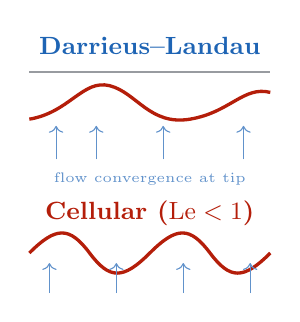
\begin{tikzpicture}[scale=0.85, font=\small]
        % DL instability sketch
        \node[font=\small\bfseries, skyblue] at (1.8,3.6)
          {Darrieus--Landau};
        % Flat flame
        \draw[thick, ashgrey!50] (0,3.2) -- (3.6,3.2);
        % Wrinked flame
        \draw[very thick, firered]
          (0,2.5)
          .. controls (0.6,2.6) and (0.8,3.1) .. (1.2,3.0)
          .. controls (1.6,2.9) and (1.8,2.4) .. (2.4,2.5)
          .. controls (3.0,2.6) and (3.2,3.0) .. (3.6,2.9);
        \draw[->, skyblue!70, thin] (0.4,1.9)--(0.4,2.4);
        \draw[->, skyblue!70, thin] (1.0,1.9)--(1.0,2.4);
        \draw[->, skyblue!70, thin] (2.0,1.9)--(2.0,2.4);
        \draw[->, skyblue!70, thin] (3.2,1.9)--(3.2,2.4);
        \node[skyblue!70, font=\tiny] at (1.8, 1.6)
          {flow convergence at tip};

        % Cellular instability
        \node[font=\small\bfseries, firered] at (1.8, 1.1)
          {Cellular ($\Le < 1$)};
        \draw[very thick, firered]
          (0,0.5)
          .. controls (0.4,0.9) and (0.6,0.9) .. (0.9,0.5)
          .. controls (1.2,0.1) and (1.4,0.1) .. (1.8,0.5)
          .. controls (2.2,0.9) and (2.4,0.9) .. (2.7,0.5)
          .. controls (3.0,0.1) and (3.2,0.1) .. (3.6,0.5);
        \draw[->,skyblue!70,thin] (0.3,-0.1)--(0.3,0.35);
        \draw[->,skyblue!70,thin] (1.3,-0.1)--(1.3,0.35);
        \draw[->,skyblue!70,thin] (2.3,-0.1)--(2.3,0.35);
        \draw[->,skyblue!70,thin] (3.3,-0.1)--(3.3,0.35);
      \end{tikzpicture}
    \end{column}
  \end{columns}
\end{frame}

% ════════════════════════════════════════════════════════════════════════
\section{Flashback and Auto-Ignition}
% ════════════════════════════════════════════════════════════════════════

\begin{frame}{Flashback: When the Flame Propagates Upstream}

  \textbf{Flashback}: local flow velocity $u_{\text{local}} < \SL$
  --- the flame propagates upstream into the fuel--air supply.

  \begin{columns}[t]
    \begin{column}{0.55\textwidth}
      \textbf{Mechanisms in LPP burners}
      \begin{enumerate}
        \item \textbf{Boundary-layer flashback}:
              $u \to 0$ at wall; flame enters boundary layer
              even when centreline $u \gg \SL$
        \item \textbf{Combustion-induced vortex breakdown
              (CIVB)}: heat release modifies the swirl velocity
              distribution, creating a reverse-flow zone
              that drags the flame upstream
        \item \textbf{Turbulent flashback}:
              local velocity fluctuations $u' > \overline{u}$
              allow instantaneous upstream penetration
      \end{enumerate}
    \end{column}
    \begin{column}{0.41\textwidth}
      \begin{alertblock}{Safety consequence}
        Flashback in a gas turbine:
        \begin{itemize}
          \item Flame enters the fuel injector / premixer
          \item Locally stoichiometric mixture burns
                inside hardware designed for premixed flow
          \item Wall temperatures exceed materials limits
                in milliseconds
          \item Potential injector burnout, structural
                failure, fuel-system fire
        \end{itemize}
      \end{alertblock}
    \end{column}
  \end{columns}
\end{frame}

\begin{frame}{Critical Velocity Gradient for Flashback}

  For a laminar boundary layer over a flat plate, the
  \textbf{critical velocity gradient} $g_c$ at the wall is:
  \[
    g_c = \frac{du}{dy}\bigg|_{\text{wall,crit}}
    \approx \frac{\SL^2}{2\alphath}
  \]

  Flashback occurs when the actual wall gradient drops below $g_c$.

  \vspace{3pt}
  \begin{columns}[t]
    \begin{column}{0.50\textwidth}
      \textbf{Prevention strategies}
      \begin{itemize}
        \item Keep mean axial velocity $\bar{u} \gg \SL$
              (low $\phi$ or high $\mdot$)
        \item Aerodynamically shaped injectors:
              avoid low-velocity corner zones
        \item Anti-flashback design: recessed injector tip
              forces flame to stabilise downstream
        \item Use non-flammable fuel--air mixture inside
              the premixer ($\phi < \phi_{\text{lean limit}}$)
      \end{itemize}
    \end{column}
    \begin{column}{0.46\textwidth}
      \begin{exampleblock}{H$_2$ challenge}
        H$_2$--air: $\SL \approx 200$ cm/s vs.\ CH$_4$--air:
        $\SL \approx 40$ cm/s.
        For hydrogen at $\phi = 0.5$: $\SL \approx 60$ cm/s.
        The required $\bar{u}$ is $\sim 5\times$ higher than
        for methane at the same condition, placing severe
        demands on injector pressure drop and swirl design.
      \end{exampleblock}
    \end{column}
  \end{columns}
\end{frame}

\begin{frame}{Auto-Ignition in Premixed Systems}

  \textbf{Auto-ignition} occurs when a premixed mixture is held above its
  auto-ignition temperature (AIT) for sufficient time.
  The ignition delay $t_{\text{ign}} \sim (c_p T_u)/(Q_{\text{HV}}\wdot_F) \propto e^{+E_a/R_u T_u}$
  decreases strongly with $T_u$.

  \begin{columns}[t]
    \begin{column}{0.50\textwidth}
      \textbf{In LPP combustors (key conflict)}
      \begin{itemize}
        \item Higher $T_3$ (compressor exit): lower $t_{\text{ign}}$
        \item Premixer residence time $\tau_{\text{premix}} =
              L_{\text{premix}}/\bar{u}$
        \item If $\tau_{\text{premix}} > t_{\text{ign}}$:
              auto-ignition inside the premixer
        \item Opposite to flashback: auto-ignition worsens
              at \emph{higher} $T_3$, flashback at \emph{higher} $\SL$
        \item Together they define a \textbf{safe operating window}
      \end{itemize}
    \end{column}
    \begin{column}{0.46\textwidth}
      \begin{alertblock}{Safe operating window}
        \centering
        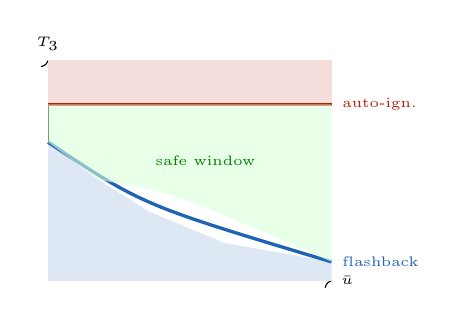
\begin{tikzpicture}[font=\small, scale=0.80]
          \draw[->] (0,0) -- (4.5,0)
            node[right,font=\tiny]{$\bar{u}$};
          \draw[->] (0,0) -- (0,3.5)
            node[above,font=\tiny]{$T_3$};
          % Auto-ignition boundary (decreasing with u)
          \fill[firered!15] (0,2.8) -- (0,3.5) -- (4.5,3.5)
            -- (4.5,2.8) -- cycle;
          \draw[firered, very thick]
            (0,2.8) -- (4.5,2.8)
            node[right,font=\tiny,firered]{auto-ign.};
          % Flashback boundary (increasing with u -- actually decreasing $u$)
          \fill[skyblue!15] (0,0) -- (0,2.2)
            -- (0.8,1.6) -- (1.6,1.1)
            -- (2.8,0.6) -- (4.5,0.3) -- (4.5,0) -- cycle;
          \draw[skyblue, very thick]
            (0,2.2) .. controls (1.5,1.2) .. (4.5,0.3)
            node[right,font=\tiny,skyblue]{flashback};
          % Safe window
          \fill[green!15, opacity=0.6]
            (0.8,1.6) .. controls (2.0,1.4) .. (4.5,0.3)
            -- (4.5,2.8) -- (0,2.8) -- (0,2.2)
            .. controls (0.4,1.9) .. (0.8,1.6);
          \node[font=\tiny, green!50!black]
            at (2.5,1.9) {safe window};
        \end{tikzpicture}
      \end{alertblock}
    \end{column}
  \end{columns}
\end{frame}

% ════════════════════════════════════════════════════════════════════════
\section{Bunsen Flame and Flame Stabilisation}
% ════════════════════════════════════════════════════════════════════════

\begin{frame}{The Bunsen Flame: Geometry and Cone Angle}

  The Bunsen burner provides the classical model for a
  \textbf{stabilised premixed flame}.

  \begin{columns}
    \begin{column}{0.44\textwidth}
      \centering
      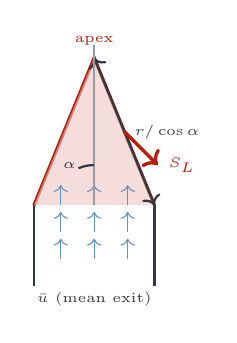
\begin{tikzpicture}[font=\small, scale=0.85]
        % Tube
        \draw[thick, ashgrey] (-0.9,-1.2) -- (-0.9,0);
        \draw[thick, ashgrey] ( 0.9,-1.2) -- ( 0.9,0);
        % Cone flame outline
        \draw[very thick, firered]
          (-0.9,0) -- (0, 2.2) -- (0.9,0);
        % Shading
        \fill[firered!25, opacity=0.6]
          (-0.9,0) -- (0,2.2) -- (0.9,0) -- cycle;
        % Velocity vectors
        \foreach \y in {-0.8,-0.4,0.0}{
          \draw[->,skyblue!70,thin] (-0.5,\y)--(-0.5,\y+0.3);
          \draw[->,skyblue!70,thin] (0.0,\y)--(0.0,\y+0.3);
          \draw[->,skyblue!70,thin] (0.5,\y)--(0.5,\y+0.3);
        }
        % Angle annotation
        \draw[<->, thick, ashgrey]
          (0.9,0) -- (0,2.2)
          node[midway, right, font=\tiny]{$r/\cos\alpha$};
        \draw[thick, ashgrey!50]
          (0,0) -- (0,2.4);
        \draw[ashgrey, thick] (0,0.6) arc (90:113:0.6)
          node[midway,left,font=\tiny]{$\alpha$};
        % Labels
        \node[firered, font=\tiny] at (0, 2.45) {apex};
        \node[ashgrey, font=\tiny] at (0,-1.4) {$\bar{u}$ (mean exit)};
        % S_L arrow (normal to cone)
        \draw[->, firered, very thick]
          (0.45,1.1) -- (0.95,0.6)
          node[right,font=\tiny,firered]{$\SL$};
      \end{tikzpicture}
    \end{column}
    \begin{column}{0.52\textwidth}
      \textbf{Geometry of the conical flame}\\[6pt]
      The flame front is stationary in the lab frame when:
      \[
        \SL = \bar{u} \sin\alpha
        \quad\Rightarrow\quad
        \sin\alpha = \frac{\SL}{\bar{u}}
      \]
      where $\alpha$ is the half-angle of the cone.

      \medskip
      This gives a direct measurement of $\SL$:
      photograph the cone angle, measure $\bar{u}$
      (Pitot tube or volumetric flow).

      \begin{block}{Area method (more accurate)}
        \[
          \SL = \frac{\dot{V}}{A_{\text{cone}}}
          = \frac{\pi r^2 \bar{u}}{\pi r \cdot r/\sin\alpha}
          = \bar{u}\sin\alpha
        \]
      \end{block}
    \end{column}
  \end{columns}
\end{frame}

\begin{frame}{Flame Stabilisation in Practical Combustors}

  A premixed flame must be \textbf{anchored} against the flow.
  The fundamental condition is:
  \[
    \text{At the stabilisation point: } u_{\text{local}} = \SL
  \]

  \begin{columns}[t]
    \begin{column}{0.50\textwidth}
      \textbf{Aerodynamic stabilisation mechanisms}
      \begin{enumerate}
        \item \textbf{Recirculation zone} (bluff body, swirl):
              hot products recirculate and continuously ignite
              fresh mixture.
              Equivalent to embedding a WSR at the base.
        \item \textbf{Pilot flame}: a small diffusion or
              rich-premixed pilot provides a hot radical pool
              to stabilise the lean main flame.
        \item \textbf{Wall attachment} (Coand\u{a} effect):
              flame anchors in the boundary layer near a
              step or recess.
      \end{enumerate}
    \end{column}
    \begin{column}{0.46\textwidth}
      \textbf{LPP gas turbine burner}
      \begin{itemize}
        \item Swirler generates a central recirculation zone (CRZ)
        \item CRZ acts as the WSR component of the
              WSR + PFR series network (Unit 5)
        \item Swirl number $S = G_\theta / (G_x r)$ controls
              CRZ size
        \item $S > 0.6$: vortex breakdown, strong CRZ
        \item Design tension: strong CRZ improves stability
              but raises residence time $\to$ more NO$_x$
      \end{itemize}
    \end{column}
  \end{columns}
\end{frame}

% ════════════════════════════════════════════════════════════════════════
\section{Summary}
% ════════════════════════════════════════════════════════════════════════

\begin{frame}{Key Equations at a Glance}
  \renewcommand{\arraystretch}{1.6}
  \begin{tabular}{>{\bfseries}p{4.0cm} p{7.5cm}}
    \toprule
    Concept & Expression \\
    \midrule
    Governing equations & $\mdot'' dY_k/dx = d(\rho D_k\,dY_k/dx)/dx
                          + \wdot_k W_k$ \\
    Flame speed (scaling) & $\SL \sim \sqrt{\alphath/\tchem}
                            \propto p^{(n-2)/2}$, $T_u^\beta$ \\
    Flame thickness & $\lf \sim \alphath/\SL = \sqrt{\alphath\,\tchem}$ \\
    Lewis number & $\Le = \alphath/D_k$; $\Le<1 \to$ instability \\
    Stretch \& Markstein & $\SL^{\text{str}} = \SL^0 - \mathcal{L}\kappa$ \\
    Quenching & $d_q \sim 4\lf$; $\Pe_{\text{crit}} \approx 40$ \\
    Flashback condition & $u_{\text{local}} < \SL$ \\
    Bunsen cone angle & $\sin\alpha = \SL/\bar{u}$ \\
    \bottomrule
  \end{tabular}
\end{frame}

\begin{frame}{Summary \& Take-Away Points}
  \begin{itemize}
    \item A laminar premixed flame is a \textbf{self-propagating
          wave} driven by the coupling of heat diffusion and
          Arrhenius chemistry.
          $\SL$ is the \emph{eigenvalue} of the governing BVP.
    \item Flame speed $\SL$ peaks near stoichiometric, decreases
          with pressure ($\propto p^{-0.1}$ for CH$_4$), and
          increases strongly with preheat temperature.
    \item The internal structure has a \textbf{thick preheat zone}
          ($\sim\lf$) and a \textbf{thin reaction zone}
          ($\sim\lf/\beta_Z$); the ZFK framework captures both.
    \item Lewis number $\Le < 1$ (H$_2$) makes flames susceptible to
          thermo-diffusive \textbf{cellular instability}.
    \item \textbf{Flashback} and \textbf{auto-ignition} define
          opposite safety limits for LPP combustors ---
          together they bound a narrow safe operating window.
    \item Flame stabilisation relies on a local $u = \SL$ balance,
          achieved in practice via a swirl-induced recirculation zone
          (WSR in the WSR + PFR series model).
  \end{itemize}
  \vfill
  \begin{center}
    \large\textbf{Next lecture:} Diffusion Flames 
  \end{center}
\end{frame}

% ── Closing slide ────────────────────────────────────────────────────
{
\setbeamertemplate{footline}{}
\setbeamertemplate{headline}{}
\setbeamercolor{background canvas}{bg=ashgrey}
\begin{frame}[plain, c]

  \begin{tikzpicture}[remember picture, overlay]
    \fill[ashgrey]
      (current page.south west) rectangle (current page.north east);
    % Flame glow bottom-right
    \fill[firered, opacity=0.15]
      (current page.south east) circle (4.5cm);
    \fill[flameyellow, opacity=0.08]
      (current page.south east) circle (2.5cm);
  \end{tikzpicture}

  \vspace{0.55cm}
  {\color{white}\fontsize{22}{26}\selectfont\bfseries
   Laminar Premixed Flames}

  \vspace{0.10cm}
  {\color{skyblue!70}\fontsize{9}{11}\selectfont
 \enspace|\enspace
  Combustion\enspace|\enspace
   }

  \vspace{0.12cm}
  
\begin{tikzpicture}
    \draw[skyblue!60, line width=0.6pt] (0,0) -- (\textwidth,0);
    \draw[firered,    line width=2.2pt] (0,0) -- (0.28\textwidth,0);
  \end{tikzpicture}

  \vspace{0.30cm}

  \begin{columns}[t, totalwidth=\textwidth]
    \begin{column}{0.315\textwidth}
      \begin{beamercolorbox}[rounded=true,wd=\linewidth,
                             sep=6pt,center]{block title}
        \textbf{\small Flame Physics}
      \end{beamercolorbox}
      \vspace{3pt}
      \begin{beamercolorbox}[rounded=true,wd=\linewidth,
                             sep=6pt,center]{block body}
        \color{ashgrey}\fontsize{7.5}{10}\selectfont
        Preheat + reaction zone structure\\[3pt]
        $\SL$ as eigenvalue of BVP\\[3pt]
        Lewis number effects\\[3pt]
        Stretch \& Markstein length
      \end{beamercolorbox}
    \end{column}
    \hfill
    \begin{column}{0.315\textwidth}
      \begin{beamercolorbox}[rounded=true,wd=\linewidth,
                             sep=6pt,center]{block title alerted}
        \textbf{\small Limits \& Instability}
      \end{beamercolorbox}
      \vspace{3pt}
      \begin{beamercolorbox}[rounded=true,wd=\linewidth,
                             sep=6pt,center]{block body alerted}
        \color{ashgrey}\fontsize{7.5}{10}\selectfont
        Lean \& rich flammability limits\\[3pt]
        Quenching distance $d_q \sim 4\lf$\\[3pt]
        Darrieus--Landau instability\\[3pt]
        Cellular flames ($\Le < 1$)
      \end{beamercolorbox}
    \end{column}
    \hfill
    \begin{column}{0.315\textwidth}
      \begin{beamercolorbox}[rounded=true,wd=\linewidth,
                             sep=6pt,center]{block title example}
        \textbf{\small Propulsion Context}
      \end{beamercolorbox}
      \vspace{3pt}
      \begin{beamercolorbox}[rounded=true,wd=\linewidth,
                             sep=6pt,center]{block body example}
        \color{white}\fontsize{7.5}{10}\selectfont
        Flashback \& auto-ignition window\\[3pt]
        Bunsen cone angle measurement\\[3pt]
        Swirl stabilisation (CRZ)\\[3pt]
        Flashback in H$_2$ LPP burners
      \end{beamercolorbox}
    \end{column}
  \end{columns}

  \vspace{0.30cm}

  \begin{beamercolorbox}[rounded=true,wd=\textwidth,
                         sep=5pt,center]{block body}
    \color{skyblue!80}\fontsize{7.8}{10}\selectfont
    $S_L \sim \sqrt{\alpha/t_{\text{chem}}}$
    \qquad\vrule width 0.4pt height 9pt depth 2pt\qquad
    $\delta_f \sim \alpha/S_L$
    \qquad\vrule width 0.4pt height 9pt depth 2pt\qquad
    $\mathrm{Le} = \alpha/D_k$
    \qquad\vrule width 0.4pt height 9pt depth 2pt\qquad
    $S_L^{\text{str}} = S_L^0 - \mathcal{L}\kappa$
    \qquad\vrule width 0.4pt height 9pt depth 2pt\qquad
    $\sin\alpha = S_L/\bar{u}$
  \end{beamercolorbox}

  \vspace{0.22cm}
  \begin{center}
    {\color{white!50}\fontsize{7.5}{9}\selectfont
     \textbf{Next:}\enspace
       Diffusion Flames}
  \end{center}

\end{frame}
}

% ════════════════════════════════════════════════════════════════════════
\appendix
\begin{frame}{Practice Problems}
  \begin{enumerate}
    \item A flat laminar CH$_4$--air flame burns at $\phi = 0.9$,
          $T_u = 300$~K, $p = 1$~atm.
          $\SL = 33$ cm/s, $\alphath = 2\times10^{-5}$ m$^2$/s.
          Estimate the flame thickness $\lf$ and the chemical
          time $\tchem$.
          Without calculation, state how each changes when
          $p$ is increased to 20 bar and explain the physical reason.

    \item Show from the scaling relation
          $\SL \sim \sqrt{\alphath/\tchem}$
          and the ideal-gas relation $\alphath \propto T_u/p$
          that $\SL \propto p^{(n-2)/2}$ for a global
          $n$-th order reaction.
          For methane ($n = 1.75$), evaluate the exponent
          and comment on whether $\SL$ is sensitive to pressure.

    \item An LPP injector premixer has length $L = 80$~mm and
          mean velocity $\bar{u} = 60$ m/s.
          The compressor exit temperature is $T_3 = 800$~K and
          $t_{\text{ign}}(800\,\text{K}) = 2$ ms for Jet-A.
          Determine whether auto-ignition occurs inside the
          premixer and whether the design is safe.
          How would doubling $\bar{u}$ affect flashback risk?

    \item Explain why a hydrogen--air LPP combustor faces
          a more challenging flashback problem than a
          methane--air combustor at the same $\phi$ and $T_3$.
          Use the Markstein number framework to also explain
          why H$_2$ flames are thermo-diffusively unstable.
  \end{enumerate}
\end{frame}

\end{document}
